\section{Applications}
Over the years EPICS has become a framework that offers users many off-the-shelf applications that ease the implementation and configuration process. Figure \ref{fig_dcs_node_msts} shows the most commonly used control-related applications. 

\begin{figure}[!h]
\centering
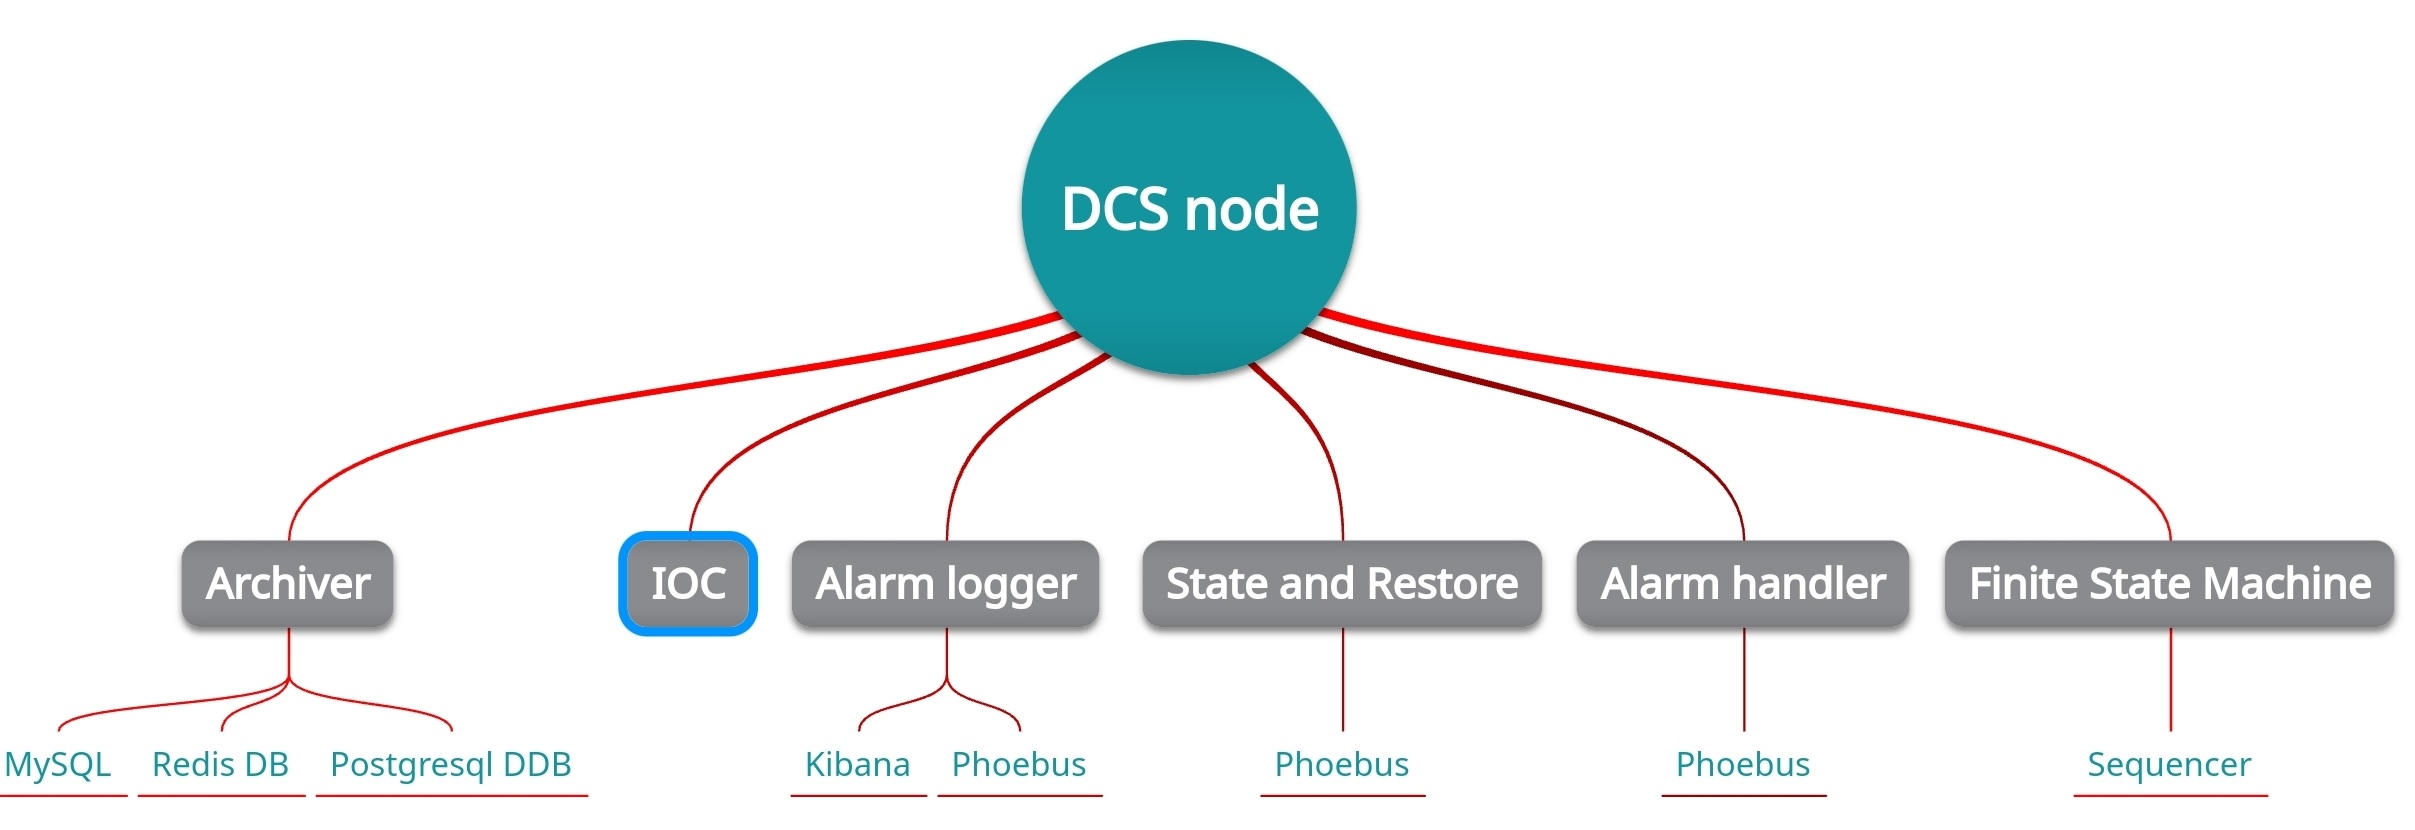
\includegraphics[width=0.95\columnwidth]{Chapter4/images/dcs_node.jpg}
\caption{Services used in addition to Phoebus functionalities}
\label{fig_dcs_node_msts}
\end{figure}
\subsection{Control System Studio and Phoebus}
Control System Studio (CS-Studio or CSS) consists of open-source Java applications and modules which can be used in constructing a control system. Phoebus is an update to the \gls{CSS} and significantly improves its performance by removing dependencies on Eclipse RCP. Phoebus uses both channel access protocol and PV access. Besides its headless applications, see below, it offers graphically based applications to access EPICS PVs, OPIs, PVs history, etc. An example of a chiller GUI is depicted in figure~\ref{fig_lauda1}. One of the main features of Phoebus is its modular nature, thanks to that users can develop and add their products or just include or exclude applications or configurations. 


\begin{figure}[!h]
\centering
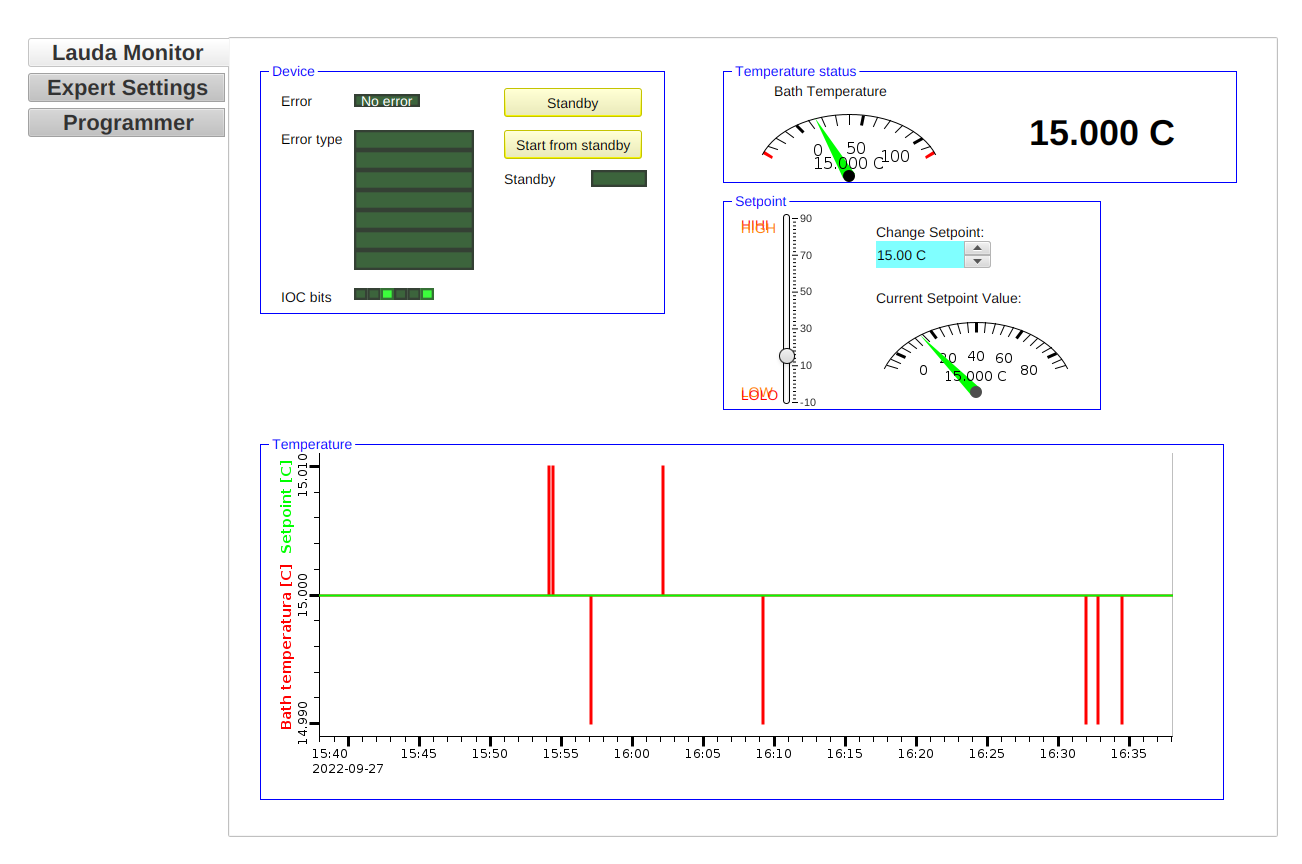
\includegraphics[width=0.9\columnwidth]{Chapter4/images/lauda1.png}
\caption{An example of a detector system \gls{GUI}}
\label{fig_lauda1}
\end{figure}

\subsection{Archiver Solutions} \label{archiver}
An Archiver serves as one of the main building blocks of the whole \gls{DCS}, as it allows the operator not only to look up the history of a given record but also to download and post-process the data. Archivers make use of the publish/subscribe logic, updating the values on change. In general, the archiver must run smoothly and without significant downtime. Moreover, the linked database and other clients should also have a stable connection with the archiver. A primary choice for STS is the so-called Archiver Appliance~\cite{archiver_appliance}. An example of the archiver appliance is divided into short-term storage, medium-term storage, and long-term storage. In principle a system administrator can adjust these settings to the needs of the specific case. Moreover, four Tomcat containers\footnote[1]{An Open source web server by the Apache foundation} are employed to handle the tasks of the archiver.  
%\begin{figure}[!h]
%\centering
%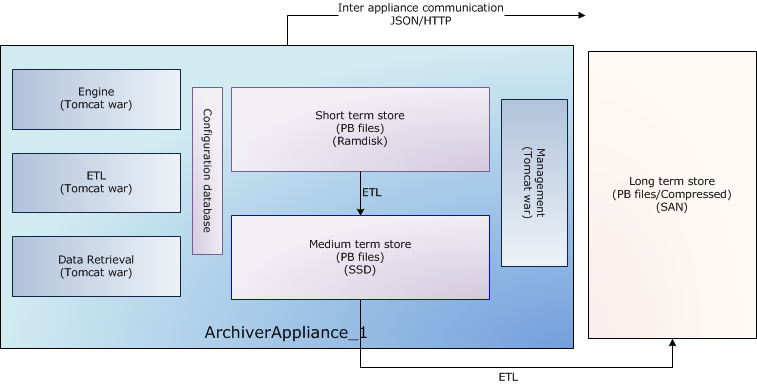
\includegraphics[width=0.7\columnwidth]{Chapter4/images/applarch.png}
%\caption{Architecture of a single appliance \cite{archiver_appliance}}
%\label{fig_archiver}
%\end{figure}
%\newline

The main advantage of the archiver include: 

\begin{itemize}
    \item Data retrieval can be integrated into Phoebus or Matlab,
    \item Wide range of supported formats/MIME types,
    \item stable performance, even with a hundred thousand \gls{PV}s
\end{itemize}
Apart from the Archiver appliance, there are also alternative solutions:

\begin{itemize}
    \item Cassandra \cite{cassandra_archive}
    \item RDB Archive engine \cite{rdb_archive}
\end{itemize}

\subsection{Alarm server}
The alarm server monitors a chosen set of \gls{PV}s, including their alarm state. EPICS records facilitate fields related to the alarm thresholds and their severity, evaluated each time the record is processed. Every numeric value could have two uppers and two lower boundaries, with assigned severities (NO\_ALARM, MINOR, MAJOR). EPICS by itself doesn't take any actions on the detector's hardware when the alarm threshold is exceeded. On the other hand, a Phoebus-based GUI will change the font color (MINOR - orange, MAJOR - red) of the variable once the alarm appears. If the connection to the alarm server exists, then the server acts upon a change in the alarm status of a record. The user interfaces show alarms, allow acknowledgment, and provide guidance and helpful links. Apache Kafka is a distributed event store and stream-processing platform which serves as a communication bus between the alarm server and Phoebus. An example of the mSTS's alarm handling is depicted in the figure~\ref{fig_alarm1}. It provides not only a visual notification of an alarm but also guidance, displays, and commands.
\begin{figure}[!h]
\centering
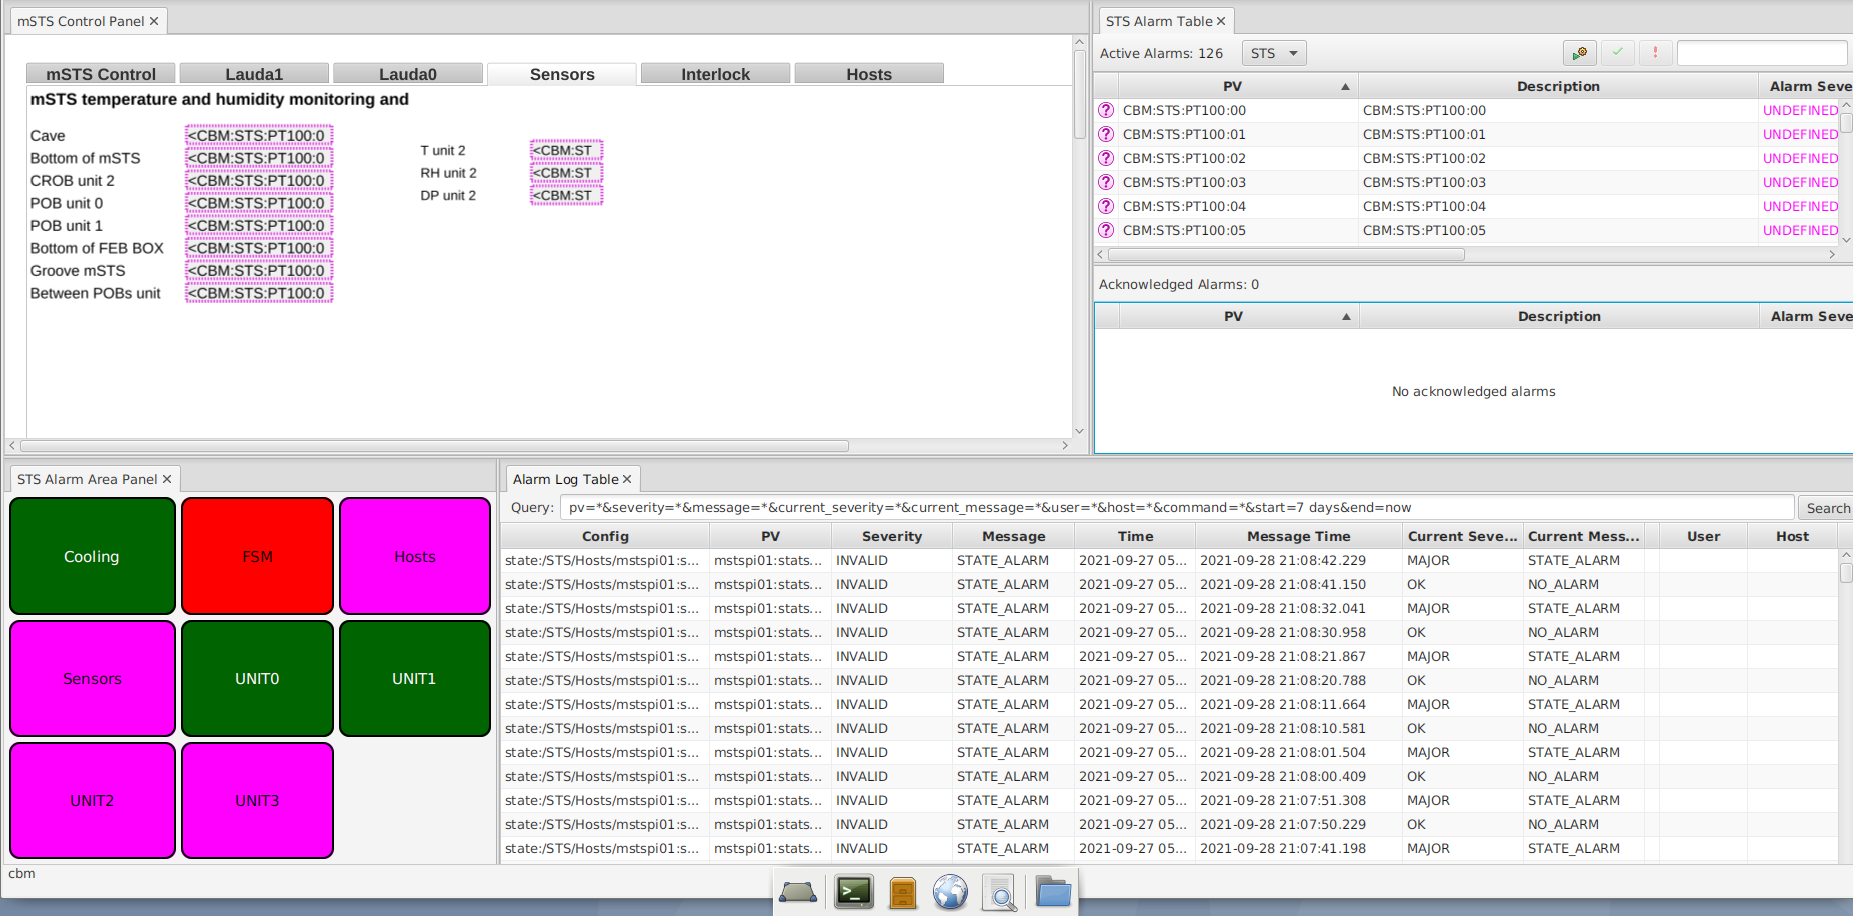
\includegraphics[width=1\columnwidth]{Chapter4/images/alarms.png}
\caption{Phoebus alarm handler view -  top left part some \gls{GUI}s, the top right part is the alarm table showing the current and acknowledged alarms, bottom left features a color status of respective nodes (e.g. cooling), bottom right shows the latest entries in the log}
\label{fig_alarm1}
\end{figure}
\newpage
\subsection{Alarm logging}
Logging is another important part of the Detector Control System. It allows monitoring and checking of all the changes in the configuration and alarms of all the process variables. Thanks to the logs acquired by the dedicated service, debugging becomes much easier. The alarm logging service enables logging of: configuration changes, state changes logging, and commands. Similarly to the alarm server, it uses Apache Kafka for data transfer. Apart from the logs \gls{GUI} available in the Phoebus \cite{alarm_logger}, an operator can also use Kibana web interface to discover patterns and trends in the data. 

\subsection{Finite state machine}
A finite state machine (\gls{FSM}) is a construct that defines states and transitions between these states. In a given moment it has a clearly defined state and a given set of rules and conditions apply to this state. An input issued by an operator or automatically by sensor(s) could trigger a transition. All transitions are unidirectional, but it's possible to define two opposite transitions, e.g. entering and escaping the error state. 

One of the possibilities to implement a \gls{FSM} is to use Sequencer, which is a State Notation Language based on C/C++. 
\begin{itemize}
    \item start-up, shut-down, fault recovery, etc
    \item little C code, many states, many transitions
    \item compiled fast can call any C++ code, easy connection to channelAccess 
\end{itemize}
One of the alternatives to the Sequencer and State Notation language is PyEPICS-based library Pysmlib. It features several interesting functions like integrated watchdog logic, multi threading, or configurable logging systems.


%\subsection{Slow control framework for small setups}
%A yaml file with all the applications became a base for several experimental setups that allowed us to expand the understanding of the hardware to be used for the STS. In the next sections of this thesis, a few main activities will be introduced, that lead to important findings. The size of the setups will differ, starting from smaller ones and progressing to larger ones. Moreover, for most of the experiments, it was not needed to deploy all of the framework components. The base of each setup was an IOC(s), which together with the database and Phoebus delivered essential information about the performed activities. 